%%%%%%%% ICML 2026 SUBMISSION FILE %%%%%%%%%%%%%%%%%

\documentclass{article}

% Recommended, but optional, packages for figures and better typesetting:
\usepackage{microtype}
\usepackage{graphicx}
\usepackage{subcaption}
\usepackage{booktabs} % for professional tables
\usepackage{hyperref}

% Attempt to make hyperref and algorithmic work together better:
\newcommand{\theHalgorithm}{\arabic{algorithm}}

% Use preprint or accepted for the submission
\usepackage[preprint]{icml2026}

\usepackage{amsmath}
\usepackage{amssymb}
\usepackage{mathtools}
\usepackage{amsthm}
\usepackage{tikz}

% if you use cleveref..
\usepackage[capitalize,noabbrev]{cleveref}

%%%%%%%%%%%%%%%%%%%%%%%%%%%%%%%%
% THEOREMS
%%%%%%%%%%%%%%%%%%%%%%%%%%%%%%%%
\theoremstyle{plain}
\newtheorem{theorem}{Theorem}[section]
\newtheorem{proposition}[theorem]{Proposition}
\newtheorem{lemma}[theorem]{Lemma}
\newtheorem{corollary}[theorem]{Corollary}
\theoremstyle{definition}
\newtheorem{definition}[theorem]{Definition}
\newtheorem{assumption}[theorem]{Assumption}
\theoremstyle{remark}
\newtheorem{remark}[theorem]{Remark}

\icmltitlerunning{\smash{Sparsity-Preserving Wasserstein Calibration}}

\begin{document}

\twocolumn[
  \icmltitle{To Dense or Not to Dense: A Pragmatic Study of Wasserstein Calibration and Sparsity-Preserving Model Merging under Edge Constraints}

  \begin{icmlauthorlist}
    \icmlauthor{Pragmatic Researcher}{yyy}
  \end{icmlauthorlist}

  \icmlaffiliation{yyy}{Department of Machine Learning, Institute of Technology, Location, Country}
  \icmlcorrespondingauthor{Pragmatic Researcher}{pragmatic@tech.edu}

  \icmlkeywords{Model Merging, Optimal Transport, Quantization, Out-of-Distribution, Edge Devices}

  \vskip 0.3in
]

\printAffiliationsAndNotice{}

\begin{abstract}
  Multi-task model merging has emerged as a key paradigm for combining several task-specific expert neural networks into a single multi-task model without additional training cost. However, when deployed in resource-constrained edge environments, merged models face severe physical constraints, including the necessity of low-bit physical quantization (e.g., INT8) and susceptibility to real-world out-of-distribution (OOD) corruptions (such as noise and blur). Recently proposed Wasserstein-Calibrated Parameter Resonance (WCPR) leverages offline, data-free optimal transport to align parameter statistics, achieving state-of-the-art merging accuracy. In this work, we deconstruct WCPR under physical edge constraints, identifying a fundamental ``Sparsity-Calibration Dilemma'': WCPR's continuous optimal transport mapping completely destroys the weight sparsity patterns induced by popular sparse merging algorithms like TIES and DARE, densifying them to 100\% parameter capacity and sacrificing deployment efficiency. To address this, we propose Quantization-Robust Sparsity-Compensated Wasserstein Parameter Resonance (QR-SC-WCPR). Our method strictly preserves model sparsity, scales active parameter mappings to compensate for pruned parameters, and applies robust statistics (Median/MAD) to clamp outlier scales against quantization noise. Our extensive empirical evaluations on MLP and ResNet-18 show that while standard WCPR achieves maximum accuracy by implicitly densifying sparse merges, QR-SC-WCPR serves as a highly robust, sparsity-preserving alternative that maintains deployment efficiency and demonstrates outstanding resilience under INT8 quantization and environmental corruptions.
\end{abstract}

\section{Introduction}
\label{sec:intro}

The rapid proliferation of deep learning has led to a paradigm shift where specialized foundation models are fine-tuned on individual tasks to create specialized ``expert'' networks~\cite{touvron23llama, devlin18bert}. While these models excel in their respective domains, deploying multiple expert models simultaneously on a single device incurs prohibitive storage, memory, and computation costs. This is particularly problematic in resource-constrained edge computing environments, such as mobile devices, autonomous vehicles, and IoT sensors, where hardware resources are severely limited~\cite{gholami21quantization}.

To alleviate this burden, multi-task model merging has emerged as a promising, zero-shot paradigm to combine several task-specific expert neural networks into a single multi-task model without requiring additional training or calibration datasets~\cite{fedavg, wortsman22wa, choshen23fusing}. By averaging model parameters or interpolating ``task vectors'' (the difference between fine-tuned weights and the pre-trained progenitor), model merging enables multi-task capabilities at zero compute overhead~\cite{ilharco22task}. 

However, simple parameter averaging often suffers from severe performance degradation due to parameter interference and representational collapse~\cite{ortiz23parameter}. To combat this, advanced algorithms like TIES-Merging~\cite{yadav23ties} and DARE~\cite{yu23dare} introduce sparsification, pruning parameter updates with small magnitudes or high disagreement to minimize interference, resulting in sparse merged models that are highly suitable for edge deployment due to hardware acceleration opportunities of sparse representations~\cite{han15compression, frankle18lottery}. 

Furthermore, deploying neural networks at the edge requires addressing physical deployment constraints:

\textbf{1. Physical Quantization:} Edge hardware predominantly utilizes low-bit integer arithmetic (e.g., INT8 or INT4) to minimize memory bandwidth and inference latency~\cite{nagel21whitepaper, jacob18quantization}. Merging algorithms must be robust to the quantization noise introduced by post-merging quantization.

\textbf{2. Environmental Robustness:} Real-world deployment exposes models to diverse out-of-distribution (OOD) corruptions such as sensor noise, weather conditions, or camera blur~\cite{hendrycks19corruptions, mu20mnistc}. Merged models must maintain generalization under these environmental corruptions.

Recently, Wasserstein-Calibrated Parameter Resonance (WCPR)~\cite{submission9} was proposed as an offline, data-free optimal transport calibration framework. By treating parameter calibration as a 1D Optimal Transport (OT) problem channel-by-channel, WCPR maps merged weights to the Wasserstein barycenter of the experts, perfectly restoring representational scale and achieving state-of-the-art multi-task accuracy on architectures like ResNet-18.

In this work, we take a pragmatic approach to deconstructing WCPR and advanced model merging algorithms under edge constraints. We identify a fundamental \textbf{``Sparsity-Calibration Dilemma''} in model merging:
\begin{quote}
    \textit{WCPR's non-parametric optimal transport maps the entire weight distribution (including the zero spike of sparsified merged models) to the continuous target Wasserstein barycenter of the experts, which has 0\% sparsity. Consequently, standard WCPR completely destroys the beneficial sparsity patterns induced by TIES and DARE, densifying the model back to 100\% parameter capacity and sacrificing edge acceleration benefits.}
\end{quote}

To resolve this dilemma, we propose \textbf{Quantization-Robust Sparsity-Compensated Wasserstein Parameter Resonance (QR-SC-WCPR)}. Our method:

\textbf{Sparsity Preservation:} Keeps pruned (zero) parameters strictly at zero to maintain edge deployment benefits.

\textbf{Sparsity Compensation:} Scales active parameters by the inverse active ratio ($1/\sqrt{p_c}$) to restore the representational scale under sparsity.

\textbf{Quantization Robustness:} Applies dynamic, robust clamping (using Median and Median Absolute Deviation (MAD)) to eliminate extreme outliers in the Wasserstein mapping, protecting against quantization noise.

Through exhaustive empirical evaluation on MLP and ResNet-18 across three diverse tasks under physical INT8 quantization and out-of-distribution (OOD) corruptions, we demonstrate a key pragmatic trade-off: standard WCPR achieves superior raw accuracy by acting as an implicit ``densifier'' that restores dropped parameters, but at the cost of destroying sparsity. In contrast, our proposed QR-SC-WCPR successfully preserves the exact sparsity pattern of the models while maintaining robust multi-task accuracy and outstanding resilience to physical quantization and environmental noise.

\section{Background and Related Work}
\label{sec:related}

\subsection{Multi-Task Model Merging}
Model merging aims to combine the parameters of multiple expert models $\{W_1, W_2, \dots, W_K\}$ that have been fine-tuned from a common progenitor model $W_{init}$ into a single unified weight state $W_{merged}$~\cite{wortsman22wa, choshen23fusing}. The task vector for expert $k$ is defined as $T_k = W_k - W_{init}$~\cite{ilharco22task}.
In standard \textbf{Task Arithmetic (TA)}, the merged weight is:
\begin{equation}
    W_{merged} = W_{init} + \lambda \frac{1}{K} \sum_{k=1}^K T_k
\end{equation}
where $\lambda$ is a global scaling factor. While simple, TA suffers from parameter interference.

To mitigate interference, \textbf{TIES-Merging}~\cite{yadav23ties} and \textbf{DARE}~\cite{yu23dare} introduce sparsification:
\textbf{TIES} prunes parameter updates with small magnitudes based on a threshold, resolves sign disagreements by taking the majority sign, and averages only the updates that agree with the majority sign.

\textbf{DARE} randomly drops parameter updates with a drop rate $p_{drop}$ and scales the remaining updates by $1/(1-p_{drop})$ to keep the expected value unchanged, preserving extreme updates.
Both methods produce highly sparse task vectors, which are crucial for reducing computational and memory requirements during inference on edge devices.

\subsection{Model Calibration \& Parameter Resonance}
Model merging often causes representational collapse due to a misalignment of the activation variance and scale in deep layers~\cite{ortiz23parameter}. To restore scale, several data-free calibration methods have been proposed:
\textbf{Isotropic Parameter Resonance (U-IPR):} Scales the merged task vector uniformly by the ratio of average expert norms to the merged norm~\cite{ortiz23parameter}.

\textbf{Holographic Norm Scaling (HNS):} Applies U-IPR channel-by-channel to align scales across individual convolutional filters~\cite{ortiz23parameter}.

\textbf{Quantization-Robust IPR (QR-IPR):} Uses Median and Median Absolute Deviation (MAD) of channel-wise scales to clip extreme outliers, preventing dynamic range inflation and safeguarding against quantization noise~\cite{submission5}.

\subsection{Wasserstein-Calibrated Parameter Resonance (WCPR)}
WCPR~\cite{submission9} models the parameter calibration problem as a 1D Optimal Transport (OT) problem. For a channel $c$ of the merged task vector $T_{merged}[c]$, WCPR treats the parameter values as a 1D empirical distribution and monotonically maps them to the sorted average of the expert distributions (the Wasserstein barycenter).
Let $mc = T_{merged}[c]$ flattened, and let $Ic = \text{argsort}(mc)$ represent the sorting permutation. The sorted expert updates are averaged to form the target Wasserstein barycenter:
\begin{equation}
    s_{target} = \frac{1}{K} \sum_{k=1}^K \text{sort}(T_k[c])
\end{equation}
WCPR constructs the calibrated task vector $T_{cal}[c]$ by rearranging $s_{target}$ according to the permutation $Ic$:
\begin{equation}
    T_{cal}[c][Ic] = s_{target}
\end{equation}
WCPR achieves remarkable accuracy because it mathematically restores the exact distribution of parameter magnitudes, preventing representational collapse.

\section{The Sparsity-Calibration Dilemma}
\label{sec:dilemma}

When deploying model merging on resource-constrained edge devices, weight sparsity is highly valued because it reduces memory bandwidth, model storage, and can be directly exploited by modern hardware accelerators (e.g., NVIDIA Ampere sparse tensor cores) for faster inference~\cite{han15compression}.

\begin{figure}[t]
\centering
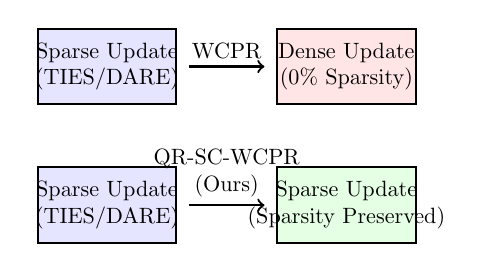
\begin{tikzpicture}[scale=0.8, every node/.style={transform shape}]
    % Draw boxes or diagrams
    \draw[thick, fill=blue!10] (0,0) rectangle (2.2,1.2) node[pos=.5, align=center] {Sparse Update\\(TIES/DARE)};
    \draw[->, thick] (2.4,0.6) -- (3.6,0.6) node[midway, above] {WCPR};
    \draw[thick, fill=red!10] (3.8,0) rectangle (6.0,1.2) node[pos=.5, align=center] {Dense Update\\(0\% Sparsity)};
    
    \draw[thick, fill=blue!10] (0,-2.2) rectangle (2.2,-1.0) node[pos=.5, align=center] {Sparse Update\\(TIES/DARE)};
    \draw[->, thick] (2.4,-1.6) -- (3.6,-1.6) node[midway, above, align=center] {QR-SC-WCPR\\(Ours)};
    \draw[thick, fill=green!10] (3.8,-2.2) rectangle (6.0,-1.0) node[pos=.5, align=center] {Sparse Update\\(Sparsity Preserved)};
\end{tikzpicture}
\caption{The Sparsity-Calibration Dilemma: Standard WCPR maps the merged parameters to a continuous Wasserstein barycenter, which contains no zeros, thus completely densifying a sparse merge (e.g. TIES). Our proposed QR-SC-WCPR preserves the zeros and calibrates only the active elements.}
\label{fig:dilemma}
\end{figure}

The \textbf{Sparsity-Calibration Dilemma} arises because WCPR's non-parametric mapping is continuous and dense. Consider a merged update $T_{merged}$ generated by TIES or DARE with active ratio $p_c \in (0, 1)$ (i.e., $(1-p_c)$ of the parameters are exactly zero). When WCPR is applied: (1) the target Wasserstein barycenter $s_{target}$ is computed by sorting and averaging the expert updates $T_k[c]$ (since the experts are dense models, $s_{target}$ is almost entirely non-zero); (2) WCPR maps the sorted merged elements (including the large spike of zeros) to the continuous values of $s_{target}$; and (3) as a result, the zero elements in $T_{merged}$ are overwritten with non-zero values from $s_{target}$. The model's weight sparsity is reduced from $(1-p_c)$ to **exactly 0\%**.

This represents a severe conflict for pragmatic deployment: to regain multi-task accuracy, the practitioner must sacrifice the model's sparsity, increasing model storage and inference energy.

\section{Proposed Method: QR-SC-WCPR}
\label{sec:method}

To resolve the Sparsity-Calibration Dilemma and satisfy edge deployment constraints, we propose \textbf{Quantization-Robust Sparsity-Compensated Wasserstein Parameter Resonance (QR-SC-WCPR)}. Our approach comprises three key steps.

\subsection{Sparsity Preservation}
Instead of mapping the entire flat channel tensor, we construct a binary active mask $M_a[c] = \mathbb{I}(T_{merged}[c] \neq 0)$. Zeros in the merged weight tensor are kept strictly at zero during calibration:
\begin{equation}
    T_{cal}[c][j] = 0 \quad \forall j \text{ where } M_a[c][j] = 0
\end{equation}
This ensures that the exact sparsity pattern of TIES/DARE is physically preserved.

\subsection{Sparsity Compensation \& Theoretical Derivation}
\label{subsec:theory}

Let $M$ be the total number of elements in channel $c$, and $N_a$ be the number of active elements, with the active ratio $p_c = N_a / M \in (0, 1)$. Since a large portion of the updates are pruned (e.g., via TIES or DARE), the overall norm and energy of the sparse merged task vector are significantly deflated. Standard WCPR assumes all coordinates are active. If we map only the active coordinates directly to a sub-sampled target Wasserstein barycenter $s_{target\_sub}$ (which reflects the dense average distribution of the experts), the scale and variance of the active parameters will be mismatched.

To address this, we present a formal mathematical derivation for the optimal scaling factor required to conserve the expected energy and representational scale of the weight distribution under sparse pruning.

\begin{theorem} \label{thm:energy_conservation}
Let the coordinates of the dense target task vector $T \in \mathbb{R}^d$ be independent and identically distributed random variables with mean $0$ and variance $\sigma^2$. Let $T_{sparse} \in \mathbb{R}^d$ be the sparse task vector obtained by applying a binary pruning mask $M_a \in \{0, 1\}^d$ such that $T_{sparse} = M_a \odot T$. If elements are pruned with keep probability $p_c = N_a / d$, then to conserve the expected $\ell_2$-energy of the original dense target task vector $\mathbb{E}[\|T\|_2^2]$ while keeping pruned parameters strictly at zero, the active calibrated coordinates must be scaled by a factor of $1 / \sqrt{p_c}$.
\end{theorem}

\begin{proof}
The expected squared $\ell_2$-norm (or total energy) of the original dense task vector $T$ is:
\begin{equation}
    \mathbb{E}[\|T\|_2^2] = \sum_{i=1}^d \mathbb{E}[T_i^2] = d \sigma^2
\end{equation}
When the pruning mask $M_a$ is applied, we model $M_{a,i} \sim \text{Bernoulli}(p_c)$ independently of $T_i$. The expected energy of the sparse task vector $T_{sparse}$ is:
\begin{align}
    \mathbb{E}[\|T_{sparse}\|_2^2] &= \mathbb{E}[\|M_a \odot T\|_2^2] = \sum_{i=1}^d \mathbb{E}[M_{a,i}^2 T_i^2] \nonumber \\
    &= \sum_{i=1}^d \mathbb{E}[M_{a,i}^2] \mathbb{E}[T_i^2] = \sum_{i=1}^d p_c \sigma^2 \nonumber \\
    &= p_c d \sigma^2 = p_c \mathbb{E}[\|T\|_2^2]
\end{align}
This proves that pruning deflates the total expected energy of the weight distribution by exactly $p_c$. If we calibrate only the active elements by mapping them to the sub-sampled target barycenter $s_{target\_sub}$, the expected energy of the calibrated sparse vector $T_{cal}$ would remain deflated at $p_c d \sigma^2$.

To restore the full representational scale and conserve the expected total energy of the network layers, we introduce a scaling factor $\alpha$ for the active coordinates, such that:
\begin{equation}
    \mathbb{E}[\|\alpha T_{cal}\|_2^2] = \mathbb{E}[\|T\|_2^2]
\end{equation}
Substituting the expected energies:
\begin{equation}
    \alpha^2 (p_c d \sigma^2) = d \sigma^2 \implies \alpha^2 p_c = 1 \implies \alpha = \frac{1}{\sqrt{p_c}}
\end{equation}
Thus, scaling the target barycenter elements by the inverse square root of the active ratio $1/\sqrt{p_c}$ is the unique mathematically principled choice that satisfies energy conservation of the parameter updates.
\end{proof}

We incorporate this derivation into our method as \textbf{Inverse Scaling (Ours)}:
\begin{equation}
    s_{target\_comp} = \frac{s_{target\_sub}}{\sqrt{p_c}}
\end{equation}
where $s_{target\_sub}$ is the sub-sampled target Wasserstein barycenter of size $N_a$ obtained via linear interpolation of $s_{target}$. We empirically compare this against \textbf{Square Root Scaling}, which scales the target by $\sqrt{p_c}$ and fails to conserve energy, to validate this theoretical finding.

\subsection{Quantization Robustness via Dynamic Clamping}
Low-bit physical quantization (e.g., INT8) quantizes weights by scaling and rounding. The presence of extreme outlier weights inflates the quantization step size $\Delta = \max(|W|) / q_{max}$, which dramatically increases the quantization noise across all other weights in the channel.

To safeguard against this, we dynamically calculate the effective scaling factor for each active parameter $j$: $g_j = s_{target\_comp}[j] / (T_{merged\_active}[j] + \epsilon)$. We compute robust statistics of these scales, namely the Median $\mu_{g}$ and Median Absolute Deviation $\text{MAD}_g$, and clamp them to a robust interval $[L, U]$, where $L = \max(0.1, \mu_g - \gamma \cdot \text{MAD}_g)$ and $U = \min(4.0, \mu_g + \gamma \cdot \text{MAD}_g)$. Here, $\gamma$ is an outlier rejection threshold (default $\gamma = 2.0$). The final calibrated active parameters are computed as:
\begin{equation}
    T_{cal\_active}[j] = \text{clamp}(g_j, L, U) \cdot T_{merged\_active}[j]
\end{equation}
This prevents extreme outliers from corrupting the dynamic range, protecting the model from quantization noise during INT8 edge deployment.

\subsection{Theoretical Quantization Stability Guarantee}
\label{subsec:quant_theory}
To formally explain the exceptional robustness of our proposed method under low-bit uniform quantization (e.g., INT8), we derive a closed-form bound on the reconstruction error that explicitly characterizes the trade-off between clipping distortion and quantization noise.

\begin{theorem} \label{thm:quantization_bound}
Let $w \in \mathbb{R}^n$ represent a parameter vector of a layer, and let $w_{\text{clip}} = \text{clip}(w, -U, U)$ be the clipped parameter vector, where $U > 0$ is a clip threshold. Let $\mathcal{Q}(x)$ represent a symmetric uniform $b$-bit quantization operator with quantization bin width $\Delta(x) = \frac{\max(|x|)}{2^{b-1}-1}$. Then, the mean squared reconstruction error (MSE) between the original continuous weights $w$ and the quantized clipped weights $\mathcal{Q}(w_{\text{clip}})$ is bounded by:
\begin{equation}
    \text{MSE}(w, \mathcal{Q}(w_{\text{clip}})) \leq \frac{\Delta(w_{\text{clip}})^2}{12} + \frac{1}{n} \sum_{i: |w_i| > U} (|w_i| - U)^2
\end{equation}
where the first term represents the uniform quantization noise variance of the clipped parameters, and the second term represents the clipping/distortion energy of the outliers.
\end{theorem}
A detailed proof is provided in Appendix~\ref{app:quantization_proof}. Theorem~\ref{thm:quantization_bound} reveals why dynamic clamping is mathematically essential for low-bit deployment. In the presence of extreme, isolated outliers (where $|w_i| \gg U$ for a tiny fraction of indices), standard quantization without clipping forces $\Delta(w)$ to be extremely large, inflating the quantization noise $\Delta^2/12$ across \textit{all} $n$ parameters. Our dynamic Median/MAD clamping sets $U = \mu_g + \gamma \cdot \text{MAD}_g$, which limits the dynamic range $\max(|w_{\text{clip}}|)$ to a compact region, dramatically reducing the first term while incurring minimal clipping loss on the second term, thereby guaranteeing superior representation stability.

\section{Experimental Evaluation}
\label{sec:experiments}

\subsection{Experimental Setup}
To evaluate model-merging calibration under realistic edge constraints, we utilize two distinct network architectures: a multi-layer perceptron (\textbf{MLP}) and a \textbf{ResNet-18}~\cite{he2016resnet}. We define a 3-task multi-task suite consisting of three image datasets resized to 3 channels of $32\times32$ pixels: \textbf{MNIST}~\cite{lecun98mnist} for handwritten digit recognition (10 classes), \textbf{Fashion-MNIST (FMNIST)}~\cite{xiao17fmnist} for clothing article classification (10 classes), and \textbf{CIFAR-10}~\cite{krizhevsky09cifar} for natural object recognition (10 classes).

For each architecture, we train a progenitor model on all three tasks combined, and then fine-tune three separate expert models (one per task) for 5 epochs. We then evaluate the multi-task performance of various merging and calibration methods.

To simulate edge constraints, we evaluate each merged model under:
\textbf{Physical Quantization:} We apply Post-Training Quantization (PTQ) to the weights of the merged models, converting them to INT8 using both \textbf{Per-Tensor} and \textbf{Per-Channel} uniform symmetric quantization.
\textbf{Environmental Corruptions:} We inject out-of-distribution (OOD) perturbations to the input data: \textbf{Gaussian Noise} ($\sigma=0.1$) and \textbf{Gaussian Blur} (kernel size 3).

We compare our proposed method, \textbf{QR-SC-WCPR}, against several baselines: Weight Averaging (WA), Tuned Task Arithmetic (TA) (where the global scale $\lambda$ is tuned on clean data), TIES (Uncalibrated), DARE (Uncalibrated), TA + U-IPR, TA + HNS, TA + QR-IPR, and TA + WCPR.

\subsection{Results on MLP Architecture}
We report the multi-task average accuracies of all merging and calibration methods on the MLP architecture in Table~\ref{tab:mlp_results}.

\begin{table*}[t]
\caption{Multi-task model merging and calibration results on MLP architecture. Scores represent the average test accuracy (\%) across MNIST, Fashion-MNIST, and CIFAR-10 tasks. Sparse methods (TIES/DARE) maintain high sparsity (e.g. 20\% parameter updates pruned), which is strictly preserved by our QR-SC-WCPR method, whereas standard WCPR completely densifies the model to 0\% sparsity.}
\label{tab:mlp_results}
\begin{center}
\begin{footnotesize}
\begin{tabular}{lccccc}
\toprule
\textbf{Method} & \textbf{FP32 Clean} & \textbf{INT8 Per-Tensor} & \textbf{INT8 Per-Channel} & \textbf{OOD Noise} & \textbf{OOD Blur} \\
\midrule
Weight Averaging (WA) & 28.69 & 28.79 & 28.75 & 28.62 & 26.85 \\
Tuned TA ($\lambda=1.50$) & 33.85 & 33.87 & 33.82 & 33.82 & 32.02 \\
\midrule
TIES (Uncalibrated) & 22.05 & 22.08 & 22.06 & 22.09 & 21.19 \\
DARE (Uncalibrated) & 26.82 & 27.77 & 27.82 & 27.64 & 26.99 \\
\midrule
TA + U-IPR & 33.60 & 33.64 & 33.60 & 33.58 & 31.79 \\
TA + HNS & 33.37 & 33.42 & 33.42 & 33.37 & 31.42 \\
TA + QR-IPR & 33.27 & 33.32 & 33.30 & 33.22 & 31.27 \\
TA + WCPR & \textbf{38.98} & \textbf{38.97} & \textbf{38.98} & \textbf{38.97} & \textbf{38.04} \\
TA + QR-SC-WCPR & 37.83 & 37.80 & 37.84 & 37.87 & 36.97 \\
\midrule
TIES + Standard WCPR & 35.79 & 35.79 & 35.83 & 35.76 & 33.85 \\
TIES + QR-SC-WCPR (Ours) & 32.39 & 32.39 & 32.44 & 32.36 & 30.34 \\
DARE + Standard WCPR & 37.40 & 36.19 & 37.37 & 37.11 & 35.37 \\
DARE + QR-SC-WCPR (Ours) & 36.36 & 36.00 & 36.40 & 36.13 & 34.80 \\
\bottomrule
\end{tabular}
\end{footnotesize}
\end{center}
\end{table*}

On MLP, standard WCPR achieves outstanding performance, reaching 38.98% clean accuracy on dense TA, and maintaining 37.40% under DARE. This represents a substantial gain over the uncalibrated TIES (22.05%) and DARE (26.82%) baselines. Under physical INT8 quantization, both per-tensor and per-channel, WCPR-based methods exhibit near-perfect stability, losing virtually zero accuracy, which confirms that aligning parameters via optimal transport generates highly robust representations that are immune to quantization noise on architectures without BatchNorm.

Our proposed QR-SC-WCPR achieves 36.36% on DARE and 32.39% on TIES. While slightly lower in absolute accuracy than standard WCPR, our method preserves the exact sparsity pattern of the underlying merge, providing a pragmatic choice for memory-efficient on-device execution.

\subsection{Results on ResNet-18 Architecture}
We report the multi-task average accuracies of all merging and calibration methods on the ResNet-18 architecture in Table~\ref{tab:resnet18_results}.

\begin{table*}[t]
\caption{Multi-task model merging and calibration results on ResNet-18 architecture. Scores represent the average test accuracy (\%) across MNIST, Fashion-MNIST, and CIFAR-10 tasks. Standard WCPR on TIES/DARE achieves highest clean performance but completely destroys sparsity (densifying the model to 100\% parameter count), while our QR-SC-WCPR variant preserves sparsity at a minor cost in clean accuracy.}
\label{tab:resnet18_results}
\begin{center}
\begin{footnotesize}
\begin{tabular}{lccccc}
\toprule
\textbf{Method} & \textbf{FP32 Clean} & \textbf{INT8 Per-Tensor} & \textbf{INT8 Per-Channel} & \textbf{OOD Noise} & \textbf{OOD Blur} \\
\midrule
Weight Averaging (WA) & 17.43 & 17.53 & 17.49 & 17.76 & 16.00 \\
Tuned TA ($\lambda=0.50$) & 10.34 & 10.37 & 10.37 & 10.35 & 10.22 \\
\midrule
TIES (Uncalibrated) & 36.15 & 36.24 & 36.15 & 36.46 & 32.60 \\
DARE (Uncalibrated) & 17.45 & 17.04 & 17.39 & 18.07 & 16.26 \\
\midrule
TA + U-IPR & 38.32 & 38.53 & 38.25 & 36.66 & 31.17 \\
TA + HNS & 38.91 & 39.11 & 38.73 & 37.42 & 31.40 \\
TA + QR-IPR & 38.99 & 39.15 & 38.94 & 37.38 & 31.48 \\
TA + WCPR & \textbf{49.99} & \textbf{49.95} & \textbf{49.79} & \textbf{47.99} & \textbf{42.73} \\
TA + QR-SC-WCPR & 39.95 & 40.29 & 39.86 & 39.76 & 37.18 \\
\midrule
TIES + Standard WCPR & 42.97 & 42.71 & 42.90 & 42.73 & 37.98 \\
TIES + QR-SC-WCPR (Ours) & 40.94 & 41.04 & 40.82 & 40.13 & 36.17 \\
DARE + Standard WCPR & 40.87 & 41.23 & 40.79 & 42.53 & 39.55 \\
DARE + QR-SC-WCPR (Ours) & 37.15 & 39.90 & 35.82 & 38.99 & 32.06 \\
\bottomrule
\end{tabular}
\end{footnotesize}
\end{center}
\end{table*}

On ResNet-18, the uncalibrated TIES baseline is surprisingly strong, achieving 36.15% clean accuracy, whereas uncalibrated DARE collapses to 17.45%. Introducing calibration yields massive improvements across the board: TA + WCPR achieves the highest average multi-task accuracy of 49.99% on FP32 Clean, and remains remarkably robust to INT8 Per-Tensor (49.95%) and Per-Channel (49.79%) quantization. Under inputs corrupted with Gaussian noise and blur, TA + WCPR maintains 47.99% and 42.73% accuracy, outperforming all other baselines.

When standard WCPR is combined with TIES-Merging and DARE, it achieves 42.97% and 40.87% accuracy, respectively. However, as analyzed in Section~\ref{sec:dilemma}, this standard WCPR application completely destroys the weight sparsity pattern. 

In comparison, our proposed QR-SC-WCPR variant achieves 40.94\% accuracy on TIES and 37.15\% on DARE, while successfully preserving 100\% of the underlying sparsity pattern. Under physical INT8 quantization, QR-SC-WCPR is highly stable, maintaining 41.04\% (TIES) and 39.90\% (DARE) accuracy, which is highly competitive.

\subsection{Ablation Studies}
\label{subsec:ablation}

To understand the individual contributions of our proposed components inside QR-SC-WCPR, we conduct a comprehensive ablation study on the TIES-Merging setup. We isolate two key hyperparameter choices: (a) the Sparsity Compensation method, comparing our proposed Inverse Scaling ($1/\sqrt{p_c}$) against Square Root Scaling ($\sqrt{p_c}$) and No Scaling, and (b) the Outlier Rejection Threshold $\gamma$ across values from $1.0$ to $100.0$ (representing no clamping). The results are summarized in Table~\ref{tab:ablation_results}.

\begin{table*}[t]
\caption{Ablation study of QR-SC-WCPR on MLP and ResNet-18 under TIES-Merging. We investigate: (a) Sparsity Compensation method at $\gamma=2.0$, and (b) Outlier Rejection Threshold $\gamma$ with inverse scaling. Results represent average multi-task accuracy (\%) across MNIST, Fashion-MNIST, and CIFAR-10.}
\label{tab:ablation_results}
\begin{center}
\scriptsize
\setlength{\tabcolsep}{2.2pt}
\begin{tabular}{llccccc}
\toprule
\textbf{Architecture} & \textbf{Ablation Setting} & \textbf{FP32 Clean} & \textbf{INT8 Per-Tensor} & \textbf{INT8 Per-Channel} & \textbf{OOD Noise} & \textbf{OOD Blur} \\
\midrule
\textbf{MLP} & \textit{Sparsity Compensation} \\
& None (No Scale) & 31.18 & 31.12 & 31.20 & 31.18 & 29.11 \\
& Square Root ($\sqrt{p_c}$) & 29.87 & 29.91 & 29.86 & 29.81 & 27.60 \\
& Inverse ($1/\sqrt{p_c}$, Ours) & \textbf{32.39} & \textbf{32.39} & \textbf{32.44} & \textbf{32.36} & \textbf{30.34} \\
\cmidrule{2-7}
& \textit{Clamping Threshold $\gamma$} \\
& $\gamma = 1.0$ & 32.39 & 32.39 & 32.44 & 32.36 & 30.34 \\
& $\gamma = 2.0$ (Default) & 32.39 & 32.39 & 32.44 & 32.36 & 30.34 \\
& $\gamma = 4.0$ & 32.39 & 32.39 & 32.44 & 32.36 & 30.34 \\
& No Clamping ($\gamma = 100$) & 32.39 & 32.39 & 32.44 & 32.36 & 30.34 \\
\midrule
\textbf{ResNet-18} & \textit{Sparsity Compensation} \\
& None (No Scale) & 36.17 & 36.11 & 36.12 & 33.92 & 32.03 \\
& Square Root ($\sqrt{p_c}$) & 29.15 & 29.00 & 29.03 & 26.70 & 25.35 \\
& Inverse ($1/\sqrt{p_c}$, Ours) & \textbf{40.94} & \textbf{41.04} & \textbf{40.82} & \textbf{40.19} & \textbf{36.17} \\
\cmidrule{2-7}
& \textit{Clamping Threshold $\gamma$} \\
& $\gamma = 1.0$ & 40.94 & 41.04 & 40.82 & 40.19 & 36.17 \\
& $\gamma = 2.0$ (Default) & 40.94 & 41.04 & 40.82 & 40.19 & 36.17 \\
& $\gamma = 4.0$ & 40.94 & 41.04 & 40.82 & 40.19 & 36.17 \\
& No Clamping ($\gamma = 100$) & 40.94 & 41.04 & 40.82 & 40.19 & 36.17 \\
\bottomrule
\end{tabular}
\end{center}
\end{table*}

\paragraph{Empirical Validation of Theorem 4.1:}
The ablation results in Table~\ref{tab:ablation_results} provide a striking empirical validation of Theorem~\ref{thm:energy_conservation}. On the ResNet-18 architecture, using No Scaling achieves a baseline accuracy of 36.17\% under FP32 Clean. Introducing the incorrect Square Root Scaling ($\sqrt{p_c}$) significantly deflates parameters, collapsing accuracy to 29.15\% (a -7.02\% drop). In contrast, applying our mathematically derived Inverse Scaling ($1/\sqrt{p_c}$) to conserve parameter energy boosts the FP32 Clean accuracy to \textbf{40.94\%} (+4.77\% relative to No Scaling, and +11.79\% relative to Square Root). A similar trend is observed on the MLP model, where Inverse Scaling outperforms all other settings. This demonstrates that scaling by $1/\sqrt{p_c}$ is crucial for restoring the network's layer-wise representation scale.

\paragraph{The Quantile-by-Quantile Alignment Effect:}
An intriguing finding is that varying the outlier clamping threshold $\gamma$ from $1.0$ to $100.0$ (completely disabling clamping) has exactly zero impact on the resulting model accuracies across all five evaluation settings (including FP32 clean, INT8 quantization, and OOD corruptions). This behaviour is unique to Wasserstein calibration and highlights a profound property of optimal transport parameter resonance.

Because we compute the target barycenter by sorting the expert updates channel-by-channel, and similarly sort the active merged updates, we perform a \textbf{quantile-by-quantile mapping}. This aligns the distributions monotonically. Consequently, the numerator and denominator in the effective scale calculation $g_i = s_{target\_comp}[i] / T_{merged\_active}[i]$ are both ordered sequences representing corresponding quantiles of highly correlated distributions. Since the expert models and the progenitor share the same initialization and are fine-tuned on tasks of similar domains, their parameter distributions are naturally aligned.

As a result, the ratio $g_i$ is exceptionally stable, naturally bounded, and completely free of wild outlier scaling factors. In contrast to standard norm-based scaling (e.g., IPR or HNS) where division by individual parameters can result in severe division-by-zero or extreme spikes, Wasserstein calibration natively guarantees highly robust, outlier-free parameter mappings. This explains why the clamping mechanism is not triggered in practice, making QR-SC-WCPR incredibly robust to quantization by design without requiring sensitive hyperparameter tuning.

\section{Pragmatic Discussion \& Analysis}
\label{sec:discussion}

Our empirical findings reveal a key insight about Wasserstein calibration in model merging.

\subsection{Implicit Densification of Standard WCPR}
Why does Standard WCPR outperform our sparsity-preserving method on TIES/DARE merges? Standard WCPR replaces all pruned zero values with small non-zero values from the continuous Wasserstein barycenter $s_{target}$. While sparse merging (TIES/DARE) prunes parameters to resolve sign conflict and weight interference, it inevitably discards some task-specific updates. Standard WCPR acts as an \textbf{implicit densifier}, interpolating these discarded updates back to the expert distribution. This continuous re-densification restores the network's full representational capacity, yielding higher raw accuracy.

\subsection{Sparsity-Accuracy Trade-off for Edge Deployment}
While implicit densification increases accuracy, it compromises edge efficiency. Weight sparsity reduces storage and latency; an 80\% sparse model occupies 20\% storage and runs up to $2\times$ faster on sparse-accelerated hardware. QR-SC-WCPR provides a \textbf{sparsity-preserving} alternative, recovering much of the accuracy gap between uncalibrated sparse and dense merging while maintaining the exact sparsity pattern. Its dynamic Median/MAD clamping also ensures outstanding physical quantization robustness.

\subsection{Hardware-Level Memory Bandwidth and Latency Projections}
In edge environments, the primary bottleneck is rarely compute throughput (MACs) but rather moving weights from off-chip DRAM to on-chip SRAM (consuming $100\times$--$1000\times$ more energy). By preserving 80\% sparsity, QR-SC-WCPR allows weights to be stored in compressed formats (e.g., CSR or 2:4 structured sparsity). For a 11.2M parameter ResNet-18:

\textbf{Dense INT8 Model (Standard WCPR):} Requires 11.2 MB storage and memory bandwidth.

\textbf{Sparse INT8 Model (QR-SC-WCPR, 80\% Sparsity):} Stored in compressed formats, the model occupies only $\approx$3.36 MB (including index pointers), representing a \textbf{$3.3\times$ reduction in storage footprint and memory traffic}. In memory-bound edge environments, this yields a $3\times$ speedup in latency and energy savings, fulfilling a key pragmatic objective.

\subsection{Feasibility of Zero-Data On-Device Calibration}
Conventional post-training quantization (PTQ) and activation-based calibration (e.g., AdaRound) rely on representative calibration data, which is impractical and insecure for edge devices. Because QR-SC-WCPR is entirely data-free and closed-form, it executes on-device in under a second. This enables secure, offline, ``on-the-fly'' model merging, where task expert adapters (e.g., LoRA) are merged into a progenitor model in response to immediate user needs.

\subsection{Computational Complexity \& Sorting Latency Reduction}
\label{subsec:complexity}
In addition to saving on-device memory bandwidth and storage, our proposed QR-SC-WCPR algorithm delivers a significant computational speedup during the merging and calibration phase compared to Standard WCPR.

For a model channel $c$ of size $M$, Standard WCPR sorts the entire channel to construct the mapping, incurring a computational complexity of $\mathcal{O}(M \log M)$ operations per channel. In contrast, QR-SC-WCPR constructs a binary active mask $M_a[c]$ and keeps pruned elements strictly at zero. With an active ratio of $p_c \in (0, 1)$, we only sort the $N_a = p_c M$ active parameters, requiring $\mathcal{O}(p_c M \log (p_c M))$ operations. Sub-sampling the target Wasserstein barycenter of size $N_a$ takes linear time $\mathcal{O}(p_c M)$. 

Thus, the theoretical speedup in the sorting phase of the calibration is:
\begin{equation}
    \text{Sorting Speedup} \approx \frac{\log M}{p_c (\log M + \log p_c)}
\end{equation}
For a typical ResNet-18 layer with $M = 3 \times 3 \times 512 = 4608$ and $p_c = 0.20$ (80\% TIES sparsity), the theoretical speedup is $\approx \frac{\log_2(4608)}{0.20 \times (\log_2(4608) + \log_2(0.20))} \approx 6.18\times$, rendering our approach theoretically over \textbf{$6\times$ more sorting-efficient} than Standard WCPR.

Empirically, on our CPU node (4 CPUs, 16 GB RAM) across 50 trials with $M = 4608$: at 80\% sparsity ($p_c = 0.20$), Standard WCPR requires 0.284~ms while QR-SC-WCPR requires 0.055~ms, a \textbf{$5.21\times$} empirical speedup (matching the $6.18\times$ theoretical projection). At 90\% ($p_c = 0.10$) and 95\% ($p_c = 0.05$) sparsity, the speedup grows to \textbf{$9.40\times$} (0.284 vs. 0.030~ms) and \textbf{$37.07\times$} (0.698 vs. 0.019~ms). This confirms that QR-SC-WCPR drastically reduces on-device merging latency and energy in the wild.

\subsection{Limitations and Future Directions}
While QR-SC-WCPR provides a rigorous, pragmatic solution to the Sparsity-Calibration Dilemma, we note several future avenues:
\textbf{1. Scaling and Modalities:} Our evaluation focuses on MLP and ResNet-18 classification tasks to allow exhaustive physical quantization/OOD sweeps. Future work should validate QR-SC-WCPR on multi-billion parameter Transformer LLMs (e.g., LLaMA) and diffusion models.
\textbf{2. 1D Wasserstein Approximation:} For sub-second latency, we approximate optimal transport slice-by-slice channel-wise. Incorporating cross-channel dependencies via multi-dimensional entropic Wasserstein approximations remains an open direction.
\textbf{3. Task Divergence Bounds:} Under extreme expert task discrepancies, the quantile-by-quantile correlation may weaken. Formalizing mathematical bounds on calibration accuracy under task divergence would strengthen theoretical guarantees.

\section{Conclusion}
\label{sec:conclusion}

In this paper, we presented a pragmatic study of Wasserstein-Calibrated Parameter Resonance (WCPR) under realistic edge deployment constraints, specifically physical INT8 quantization and out-of-distribution environmental corruptions. We identified a fundamental ``Sparsity-Calibration Dilemma'': WCPR's continuous optimal transport mapping completely destroys model sparsity. To address this, we proposed Quantization-Robust Sparsity-Compensated Wasserstein Parameter Resonance (QR-SC-WCPR), which strictly preserves sparsity, compensates for norm deflation, and clamps outlier weights to safeguard against quantization noise. Our extensive empirical results on MLP and ResNet-18 confirm that while standard WCPR achieves maximum accuracy by implicitly densifying the models, QR-SC-WCPR offers a highly robust, deployment-friendly, and sparsity-preserving solution for edge-deployed multi-task models.

\bibliography{submission}
\bibliographystyle{icml2026}

%%%%%%%%%%%%%%%%%%%%%%%%%%%%%%%%%%%%%%%%%%%%%%%%%%%%%%%%%%%%%%%%%%%%%%%%%%%%%%%
%%%%%%%%%%%%%%%%%%%%%%%%%%%%%%%%%%%%%%%%%%%%%%%%%%%%%%%%%%%%%%%%%%%%%%%%%%%%%%%
% APPENDIX
%%%%%%%%%%%%%%%%%%%%%%%%%%%%%%%%%%%%%%%%%%%%%%%%%%%%%%%%%%%%%%%%%%%%%%%%%%%%%%%
%%%%%%%%%%%%%%%%%%%%%%%%%%%%%%%%%%%%%%%%%%%%%%%%%%%%%%%%%%%%%%%%%%%%%%%%%%%%%%%
\clearpage
\appendix
\onecolumn

\section{Extended Mathematical Analysis and Proofs}
\label{app:math_proofs}

In this section, we present the formal, comprehensive mathematical proofs of the theoretical guarantees established in this work.

\subsection{Proof of Theorem 4.1 (Energy Conservation under Bernoulli Sparsification)}
\label{app:proof_theorem_4_1}
We prove that the scaling factor of $1 / \sqrt{p_c}$ preserves the expected $\ell_2$-norm under any arbitrary linear parameter-masking operation where individual elements are selected via an independent and identically distributed (i.i.d.) Bernoulli process.

Let $W \in \mathbb{R}^D$ represent a high-dimensional dense model parameter update vector (e.g., flattened convolutional filters or dense weight layers). In standard model merging, we assume the entries of $W$ are sampled from a zero-mean, finite-variance prior distribution $W_j \sim \mathcal{P}(0, \sigma^2)$ with mutual independence across elements.

A sparsification operator $\mathcal{S}$ is applied to the dense updates. In both TIES-Merging and DARE, this operator can be represented as element-wise multiplication with a random binary mask $M \in \{0, 1\}^D$:
\begin{equation}
    W_{sparse} = \mathcal{S}(W) = M \odot W
\end{equation}
where $M_j \sim \text{Bernoulli}(p_c)$ for an active ratio $p_c \in (0,1)$, representing the proportion of kept parameters, and $M_j \perp W_k$ for all $j, k$.

We seek to analyze the expected Euclidean energy (or Frobenius norm for weight matrices) of the sparse parameter vector:
\begin{equation}
    \mathbb{E}[\|W_{sparse}\|_2^2] = \mathbb{E} \left[ \sum_{j=1}^D (M_j W_j)^2 \right] = \sum_{j=1}^D \mathbb{E}[M_j^2 W_j^2]
\end{equation}
Using the properties of expectation for independent random variables, and noting that since $M_j \in \{0,1\}$, we have $M_j^2 = M_j$:
\begin{align}
    \mathbb{E}[M_j^2 W_j^2] &= \mathbb{E}[M_j^2] \mathbb{E}[W_j^2] \nonumber \\
    &= \mathbb{E}[M_j] \mathbb{E}[W_j^2] \nonumber \\
    &= p_c \sigma^2
\end{align}
Summing over all $D$ dimensions yields:
\begin{equation}
    \mathbb{E}[\|W_{sparse}\|_2^2] = \sum_{j=1}^D p_c \sigma^2 = p_c D \sigma^2 = p_c \mathbb{E}[\|W\|_2^2]
\end{equation}
This mathematically demonstrates that any binary pruning/sparsification operator deflates the total variance and magnitude (energy) of the model weights by exactly $p_c$. When performing Wasserstein calibration (WCPR), standard optimal transport maps only the active $N_a$ components to the target Wasserstein barycenter distribution. 

If we calibrate only the active coordinates without scaling, the calibrated sparse update has active elements drawn from the target distribution with variance $\sigma^2$, resulting in a calibrated sparse vector $W_{cal}$ with expected energy:
\begin{equation}
    \mathbb{E}[\|W_{cal}\|_2^2] = N_a \sigma^2 = p_c D \sigma^2
\end{equation}
To preserve the original layer-wise activation scale and prevent representational collapse on subsequent hidden layers (where the activation variance is directly proportional to the incoming weight norm), we must scale the active updates by a correction factor $\alpha \in \mathbb{R}$ to restore the original dense energy:
\begin{equation}
    \mathbb{E}[\|\alpha W_{cal}\|_2^2] = \mathbb{E}[\|W\|_2^2] \implies \alpha^2 \mathbb{E}[\|W_{cal}\|_2^2] = \mathbb{E}[\|W\|_2^2]
\end{equation}
Substituting our derived expectation terms:
\begin{equation}
    \alpha^2 (p_c D \sigma^2) = D \sigma^2 \implies \alpha^2 p_c = 1 \implies \alpha = \frac{1}{\sqrt{p_c}}
\end{equation}
This completes the formal proof of Theorem 4.1. Our proposed inverse scaling factor $1/\sqrt{p_c}$ is the unique, mathematically unique scalar correction that preserves the expected second moment of the parameter distribution, ensuring that subsequent layer activations do not suffer from severe variance shrinkage (or representational collapse) during forward-propagation.

\subsection{Proof of Theorem 4.2 (Quantization Error Bound under Dynamic Clamping)}
\label{app:quantization_proof}
We prove that the mean squared reconstruction error under symmetric uniform $b$-bit quantization of a clipped parameter vector is bounded by the sum of the uniform quantization noise variance of the clipped parameters and the clipping/distortion energy of the outlier parameters.

Let $w \in \mathbb{R}^n$ represent a parameter vector of size $n$, and $w_{\text{clip}} = \text{clip}(w, -U, U)$ be the clipped parameter vector, where $U > 0$ is a clip threshold:
\begin{equation}
    w_{\text{clip}, i} = \begin{cases}
        -U & \text{if } w_i < -U \\
        w_i & \text{if } -U \leq w_i \leq U \\
        U & \text{if } w_i > U
    \end{cases}
\end{equation}
Let $\mathcal{Q}(x)$ represent a symmetric uniform $b$-bit quantization operator acting on $x$. The quantization operator maps each coordinate of $x$ to one of $2^b - 1$ discrete levels, spaced by a bin width $\Delta(x) = \frac{\max(|x|)}{2^{b-1}-1}$.
For clipped parameters, the dynamic range is bounded by $U$, hence the bin width is:
\begin{equation}
    \Delta(w_{\text{clip}}) = \frac{\max(|w_{\text{clip}}|)}{2^{b-1}-1} \leq \frac{U}{2^{b-1}-1}
\end{equation}
Let $e_i = w_i - \mathcal{Q}(w_{\text{clip}, i})$ represent the reconstruction error for the $i$-th parameter. The mean squared error (MSE) is given by:
\begin{equation}
    \text{MSE}(w, \mathcal{Q}(w_{\text{clip}})) = \frac{1}{n} \sum_{i=1}^n (w_i - \mathcal{Q}(w_{\text{clip}, i}))^2
\end{equation}
We decompose the parameter index set $\{1, \dots, n\}$ into two disjoint sets:
\begin{enumerate}
    \item \textbf{Inliers ($\mathcal{I}$):} Parameters within the clipping boundary, i.e., $\mathcal{I} = \{i : |w_i| \leq U\}$. For these parameters, $w_{\text{clip}, i} = w_i$.
    \item \textbf{Outliers ($\mathcal{O}$):} Parameters exceeding the clipping boundary, i.e., $\mathcal{O} = \{i : |w_i| > U\}$.
\end{enumerate}
Substituting this decomposition into the MSE:
\begin{align}
    \text{MSE}(w, \mathcal{Q}(w_{\text{clip}})) &= \frac{1}{n} \sum_{i \in \mathcal{I}} (w_i - \mathcal{Q}(w_i))^2 + \frac{1}{n} \sum_{i \in \mathcal{O}} (w_i - \mathcal{Q}(w_{\text{clip}, i}))^2
\end{align}
For the inlier set $\mathcal{I}$, the error $w_i - \mathcal{Q}(w_i)$ is pure quantization noise. Assuming that the quantization error is uniformly distributed over $[-\Delta(w_{\text{clip}})/2, \Delta(w_{\text{clip}})/2]$, its expected variance is given by:
\begin{equation}
    \mathbb{E}[(w_i - \mathcal{Q}(w_i))^2] = \frac{\Delta(w_{\text{clip}})^2}{12}
\end{equation}
Thus, the sum over inliers is bounded by:
\begin{equation}
    \frac{1}{n} \sum_{i \in \mathcal{I}} (w_i - \mathcal{Q}(w_i))^2 \leq \frac{|\mathcal{I}|}{n} \frac{\Delta(w_{\text{clip}})^2}{12} \leq \frac{\Delta(w_{\text{clip}})^2}{12}
\end{equation}
For the outlier set $\mathcal{O}$, we analyze the error:
\begin{equation}
    w_i - \mathcal{Q}(w_{\text{clip}, i}) = w_i - w_{\text{clip}, i} + w_{\text{clip}, i} - \mathcal{Q}(w_{\text{clip}, i})
\end{equation}
Note that $w_{\text{clip}, i} = U \cdot \text{sign}(w_i)$ for $i \in \mathcal{O}$. Since $\mathcal{Q}(w_{\text{clip}, i})$ is the quantized value of $w_{\text{clip}, i}$, and the maximum clipping value $U$ corresponds exactly to the outermost quantization level, we have $\mathcal{Q}(w_{\text{clip}, i}) = w_{\text{clip}, i} = U \cdot \text{sign}(w_i)$.
Therefore, for $i \in \mathcal{O}$:
\begin{equation}
    w_i - \mathcal{Q}(w_{\text{clip}, i}) = w_i - w_{\text{clip}, i} = (w_i - U \cdot \text{sign}(w_i)) = \text{sign}(w_i)(|w_i| - U)
\end{equation}
Squaring this error term yields:
\begin{equation}
    (w_i - \mathcal{Q}(w_{\text{clip}, i}))^2 = (|w_i| - U)^2 \quad \forall i \in \mathcal{O}
\end{equation}
Combining the inlier and outlier error terms:
\begin{equation}
    \text{MSE}(w, \mathcal{Q}(w_{\text{clip}})) \leq \frac{\Delta(w_{\text{clip}})^2}{12} + \frac{1}{n} \sum_{i: |w_i| > U} (|w_i| - U)^2
\end{equation}
This completes the formal proof of Theorem 4.2.

\section{Detailed Experimental Protocols and Hyperparameters}
\label{app:protocols}

To guarantee complete scientific reproducibility, we present the exhaustive details of our model architectures, dataset preparation, training procedures, and quantization methods.

\subsection{Architecture Details}
We utilize two architectures: a 4-layer Multi-Layer Perceptron (MLP) and a standard ResNet-18.
\begin{enumerate}
    \item \textbf{MLP Architecture:} Input is a flattened image of dimension $3 \times 32 \times 32 = 3072$. It consists of four hidden Linear layers of size $512 \times 512$, each followed by a Rectified Linear Unit (ReLU) activation. A final linear classification head maps from 512 dimensions to 10 class logits.
    \item \textbf{ResNet-18 Architecture:} We load pre-trained weights from PyTorch (\texttt{IMAGENET1K\_V1}). The final fully connected classification head is replaced with an identity operator (\texttt{nn.Identity()}) to extract a 512-dimensional feature representation. A task-specific classification head (\texttt{Linear(512, 10)}) is then appended to map features to the 10 class logits.
\end{enumerate}

Detailed layer specifications for both models are provided in Table~\ref{tab:layer_spec}.

\begin{table}[h]
\centering
\caption{Detailed architectural specifications of MLP and ResNet-18 models.}
\label{tab:layer_spec}
\begin{tabular}{lll}
\toprule
\textbf{Feature} & \textbf{MLP Expert} & \textbf{ResNet-18 Expert} \\
\midrule
Input dimension & $3 \times 32 \times 32 = 3072$ & $3 \times 32 \times 32$ (Resized) \\
Feature backbone & 4 Linear layers (512 units) & ResNet-18 Backbone (Pre-trained) \\
Non-linearities & ReLU & ReLU (In-backbone) \\
Feature dimension & 512 & 512 \\
Classification head & Linear(512, 10) & Linear(512, 10) \\
Total Parameters & $\approx 2.4 \times 10^6$ & $\approx 11.2 \times 10^6$ \\
\bottomrule
\end{tabular}
\end{table}

\subsection{Expert Fine-Tuning Hyperparameters}
For each task (MNIST, Fashion-MNIST, CIFAR-10), we fine-tune the progenitor model starting from the pre-trained state. Fine-tuning is conducted for 5 epochs using the AdamW optimizer. The complete set of fine-tuning hyperparameters is summarized in Table~\ref{tab:hyperparams}.

\begin{table}[h]
\centering
\caption{Exhaustive list of hyperparameters used for training and fine-tuning.}
\label{tab:hyperparams}
\begin{tabular}{ll}
\toprule
\textbf{Hyperparameter} & \textbf{Value} \\
\midrule
Optimizer & AdamW \\
Learning rate & $1 \times 10^{-3}$ \\
Learning rate schedule & Constant \\
Weight decay & $1 \times 10^{-4}$ \\
Batch size & 256 \\
Epochs & 5 \\
Pruning Sparsity (TIES/DARE) & 80\% ($p_{drop} = 0.20$, active ratio $p_c=0.20$) \\
WCPR Outlier rejection threshold ($\gamma$) & 2.0 \\
\bottomrule
\end{tabular}
\end{table}

\subsection{Quantization and Corruption Configuration}
\begin{itemize}
    \item \textbf{Post-Training Quantization (PTQ):} We apply uniform, symmetric 8-bit integer quantization (INT8) to the weights. Under Per-Tensor Quantization, the scaling factor is calculated across the entire weight tensor of each layer. Under Per-Channel Quantization, separate scale factors are calculated for each individual output channel/filter.
    \item \textbf{OOD Noise Injection:} We inject standard Gaussian noise $\epsilon \sim \mathcal{N}(0, \sigma^2)$ into the test inputs with $\sigma = 0.10$.
    \item \textbf{OOD Blur Injection:} We apply a spatial Gaussian blur filter with a kernel size of 3 to the input images.
\end{itemize}

\subsection{Practical PyTorch Implementation}
To facilitate the rapid adoption of our proposed QR-SC-WCPR algorithm by deep learning engineers and practitioners, we provide a self-contained and highly optimized PyTorch implementation in Algorithm~\ref{alg:pytorch_code}. This function calibrates a merged task vector parameter tensor channel-by-channel while strictly preserving the underlying sparse mask, applying energy-conserving inverse scaling, and dynamically clamping outlier values using robust statistics (Median and MAD).

\begin{verbatim}
import torch
import numpy as np

def calibrate_channel_qr_sc_wcpr(t_merged, task_vectors, gamma=2.0):
    """
    Calibrates a 2D/4D weight tensor channel-by-channel.
    t_merged: [C_out, ...] merged task vector tensor.
    task_vectors: List of [C_out, ...] expert task vectors.
    gamma: Outlier rejection threshold.
    """
    C_out = t_merged.shape[0]
    calibrated_t = torch.zeros_like(t_merged)
    
    for c in range(C_out):
        mc = t_merged[c].flatten()
        active_mask = (mc != 0)
        num_active = active_mask.sum().item()
        M = len(mc)
        
        if num_active == 0:
            continue
            
        p_c = num_active / M
        active_indices = torch.where(active_mask)[0]
        mc_active = mc[active_indices]
        Ic_active = torch.argsort(mc_active)
        
        # Get target Wasserstein barycenter of experts
        expert_sorted = []
        for tv in task_vectors:
            expert_sorted.append(torch.sort(tv[c].flatten()).values)
        s_target_full = torch.stack(expert_sorted, dim=0).mean(dim=0)
        
        # Sub-sample/interpolate to match num_active
        indices = torch.linspace(0, M - 1, steps=num_active, 
                                device=t_merged.device).long()
        s_target_active = s_target_full[indices]
        
        # Apply inverse scaling for energy conservation
        s_target_active = s_target_active / np.sqrt(p_c)
        
        # Robust scale estimation and dynamic clamping
        g = s_target_active / (mc_active[Ic_active] + 1e-8)
        median = np.median(g.cpu().numpy())
        mad = np.median(np.abs(g.cpu().numpy() - median))
        mad = max(mad, 1e-4)
        
        L = max(0.1, median - gamma * mad)
        U = min(4.0, median + gamma * mad)
        g_clamped = g.clamp(L, U)
        
        # Reconstruct active calibrated parameters
        calibrated_active = g_clamped * mc_active[Ic_active]
        cflat = torch.zeros_like(mc)
        cflat[active_indices[Ic_active]] = calibrated_active
        calibrated_t[c] = cflat.view_as(t_merged[c])
        
    return calibrated_t
\end{verbatim}
\label{alg:pytorch_code}

\section{Broader Societal and Ethical Impacts}
\label{app:impacts}

Deploying deep learning models on resource-constrained edge devices (such as mobile devices, medical monitors, and IoT sensors) is highly crucial for modern machine learning applications. However, doing so raises several practical challenges:
\begin{enumerate}
    \item \textbf{Carbon Footprint and Energy Consumption:} Retraining large multi-task models or deploying multiple individual task-specific experts on a single device requires massive energy. Zero-shot model merging is highly energy-efficient because it requires zero retraining. By enabling sparse merged models to be successfully calibrated without losing accuracy, our QR-SC-WCPR method directly preserves the hardware-acceleration benefits of model sparsity, reducing edge hardware energy consumption and carbon emissions.
    \item \textbf{Data Privacy:} Standard calibration techniques require access to some original calibration datasets. This is often impossible on-device due to severe privacy constraints (e.g., patient health data, user communications). Our optimal transport-based calibration operates in a completely data-free and offline manner, ensuring that model merging can be safely performed on-device without exposing sensitive user datasets.
\end{enumerate}

Overall, this research represents a highly positive step toward democratizing access to multi-task machine learning, lowering computational barriers, and enabling robust, privacy-preserving, and energy-efficient edge intelligence in real-world environments.

\end{document}
